\chapter{The Impact of AGN on Ly\texorpdfstring{$\alpha$}{a} Emission from Massive Halos}
\label{sec:agn}

We now turn our attention to the influence of an AGN on our modeled Ly$\alpha$ emission.
We note that we do not explicitly include AGN feedback; instead, from the perspective of the hydrodynamic simulations, black holes are included as passive sink particles that only accrete (\S~\ref{sec:methods}).
This said, we are able to assess their impact on the emission properties of the simulations in postprocessing.
Here, we treat AGN as an ionizing source when we compute the ionization state of the gas with {\sc lycrt}.
In this model, the AGN SED is modeled by employing the \citet*{Hopkins2007} templates for unreddened quasars, with the luminosity being tied to the accretion rate via $L = \eta \dot{M_{\rm BH}} c^2$, where $\eta$ is an efficiency parameter with a fiducial value of $\eta = 0.1$.
In what follows,  we investigate the impact of AGN on the total Ly$\alpha$ luminosity, as well as the overall spatial extent of the blob.

%We also investigate the effect of introducing ionization due to AGN emission. In our model, AGN only behave as a source of ionization when we compute the state of the gas, so their primary effect is to ionize a large amount of gas and boost the emission due to recombination (Figure~\ref{fig:agn_comparison}).

\section{Impact of AGN on Luminosity and Escape Fraction}
In Figure~\ref{fig:agn_comparison}, we plot a comparison of the time evolution of the Ly$\alpha$ luminosity, escape fraction, and ionized gas fraction for models with and without an AGN for our fiducial galaxy.  As is evident, there are significant differences in a model that includes AGN compared to one that does not.

Since Ly$\alpha$ escape is sightline-dependent we show in Figure~\ref{fig:f_esc} the variation of our fiducial LAB's luminosity and escape fraction over sightlines, with ionization due to AGN and without.
The total luminosity can vary substantially due to the viewing angle of the galaxy when AGN are present.
To demonstrate this explicitly, in the top panel of Figure~\ref{fig:f_esc}, we plot the maximum relative variation between sightlines to show how different a single physical object may appear to an observer who can only view the object from one line of sight.
This huge variation when AGN are present is caused by the distinct non-uniformity of CGM opacity; it's as if the AGN punches large ionization holes in the enclosing CGM through which Ly$\alpha$ readily escapes.
It is important to note that the distribution of escape fractions is not normal, we sample 3072 sightlines to produce this plot which is sufficient to explore all the high-escape pathways out of a LAB.
The top panel of Figure~\ref{fig:f_esc} shows how much variation is possible, and how much the presence of these high-escape sightlines varies over redshift, and the bottom plot shows how dispersed the typical sightlines are.
Because of this sightline variation, an escape fraction (or luminosity) calculated along a single line of sight may not be particularly representative of the overall galaxy properties.

When we include a model for AGN (which drives increased ionization in the gas), there are substantial spikes in the luminosity owing to increased emission from recombinations.  In short, the primary effects are to increase the Ly$\alpha$ luminosity owing to an increase in the ionization fraction of the gas.  As we recall from Section~\ref{sec:physicalconcepts}, as we increase the ionization state of the gas at a fixed temperature (say $T=10^4$ K), the  luminosity from recombinations increases while that from collisional excitations decreases.  Additionally, the escape fraction increases with the addition of an AGN (middle panel of Figure~\ref{fig:agn_comparison}), due to the fact that the Ly$\alpha$ scattering strength depends primarily on $n_{\HI}$ (Equation~\ref{eq:kalpaha}).   This escape fraction enhancement is so substantial than at some orientation angles we can see $f_{\rm esc} > 1$.   due to particular geometries that cause Ly$\alpha$ to scatter into the line of sight more than it is absorbed.

Taken together, the increase in the ionization state of the gas (bottom panel of Figure~\ref{fig:agn_comparison}) increases both the emission from recombinations, as well as the escape fraction of Ly$\alpha$ photons. These combined effects allow for significant boosting ($\sim$ factors of $10-50$) of the Ly$\alpha$ luminosity compared to a no-AGN model.

\begin{figure}
    \centering
    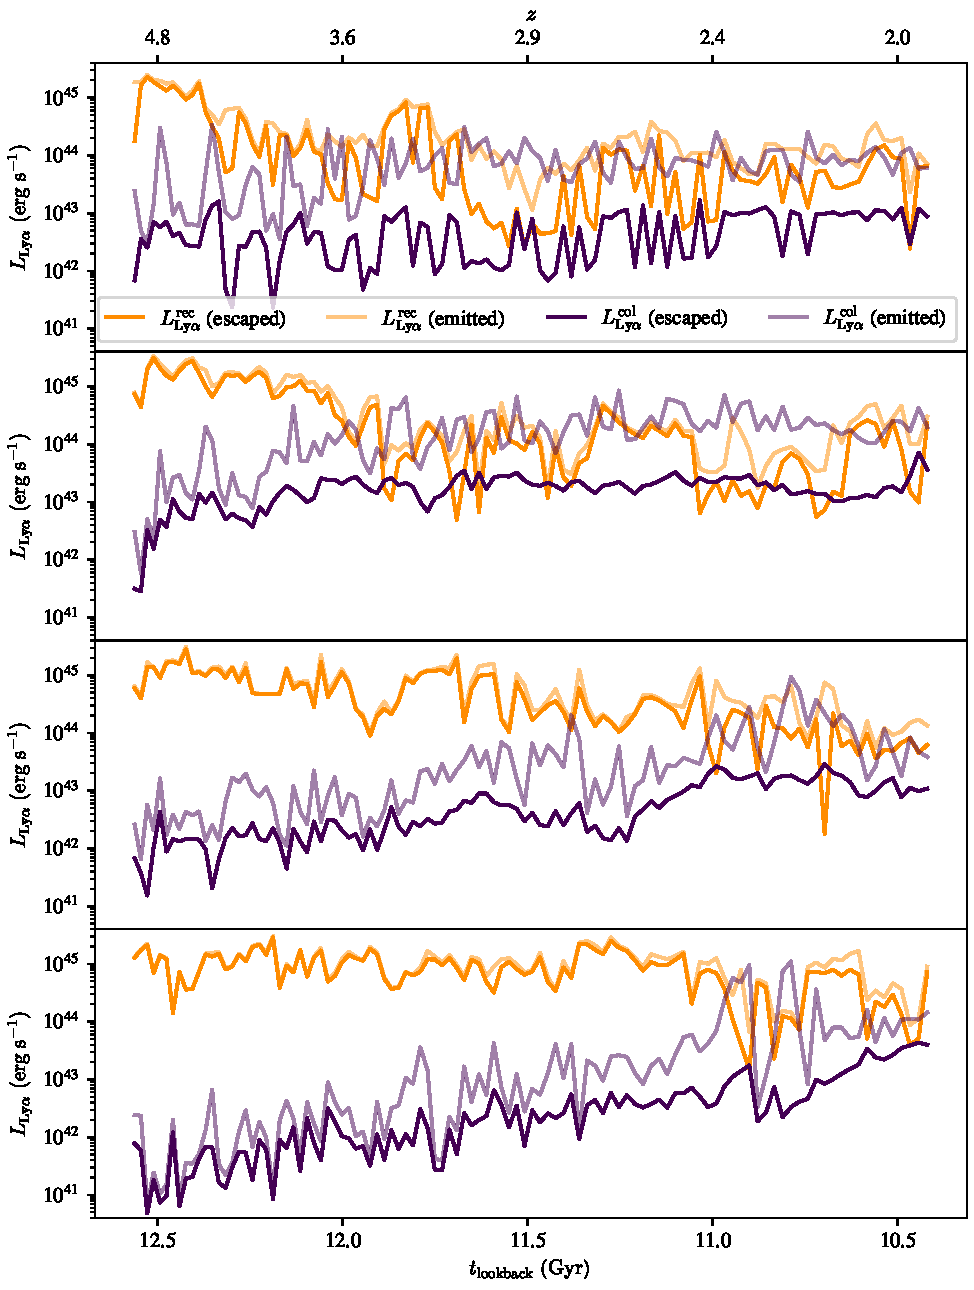
\includegraphics[width=\textwidth,height=\textheight,keepaspectratio]{figures/agn_recombination_collision.pdf}
    \caption{All our snapshots broken down by source of emission over redshift; as opposed to Figure~\ref{fig:recombination_collision} this plot includes the effect of AGN.}
    \label{fig:agn_recombination_collision}
\end{figure}

%The emission of our model is sometimes massively dominated by emission from recombinations, but when we remove AGN from the model in Figure~\ref{fig:agn_comparison}, the spikes in luminosity disappear. This AGN-driven luminosity is due to a change in the ionization state of the gas (Figure~\ref{fig:agn_comparison}); recall from Section~\ref{sec:physicalconcepts} that recombination increases (for $T \leq 10^4$ K) as we ionize the gas and emission from collisional excitations declines. In addition, the ionization from adding AGN to the model increases the Ly$\alpha$ escape fraction (Figure~\ref{fig:agn_comparison}) because Ly$\alpha$ scattering only depend on $n_{HI}$ (Eq.~\ref{eq:kalpaha}). This escape fraction enhancement is so substantial than at some orientation angles we can see $f_{esc} > 1$ (Figure~\ref{fig:f_esc}). This $f_{esc} > 1$ is produced by particular geometries that cause Ly$\alpha$ to scatter into the line of sight more than it is absorbed.

\begin{figure}
  \centering
    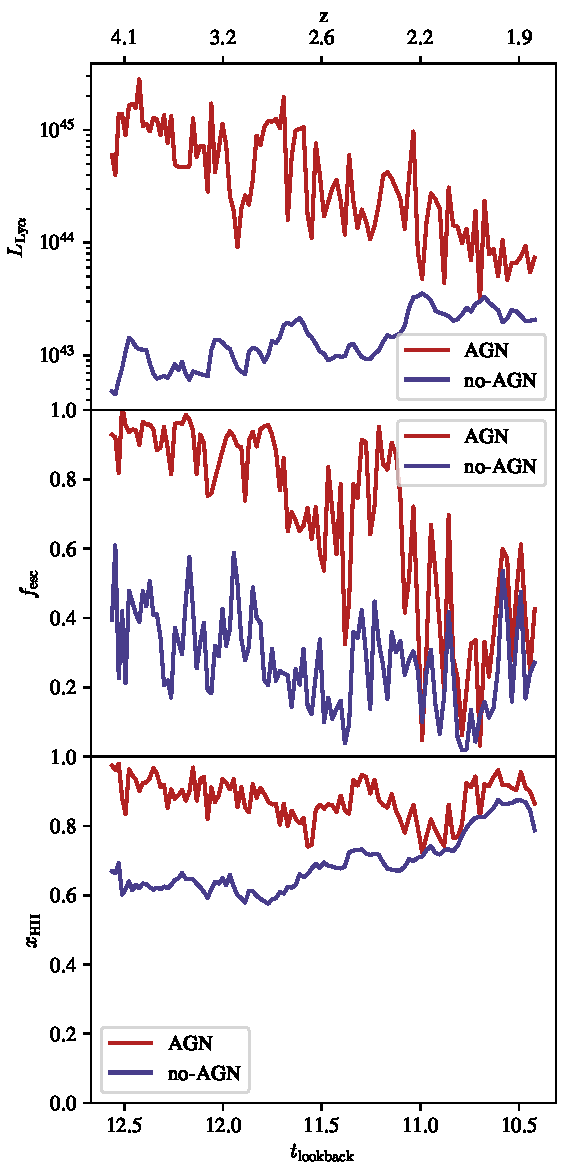
\includegraphics[width=\textwidth,height=\textheight,keepaspectratio]{figures/agn_comparison.pdf}
  \caption{We compare the luminosity, escape fraction, and ionization state of the galaxy and halo with and without an AGN model. The luminosity of a Ly$\alpha$ blob is sometimes substantially enhanced by the AGN model. The simulation domain is always heavily ionized, but the presence of AGN also provides stochastic enhancements, though it does not well correlate with luminosity or escape.}
  \label{fig:agn_comparison}
\end{figure}

\begin{figure}
    \centering
    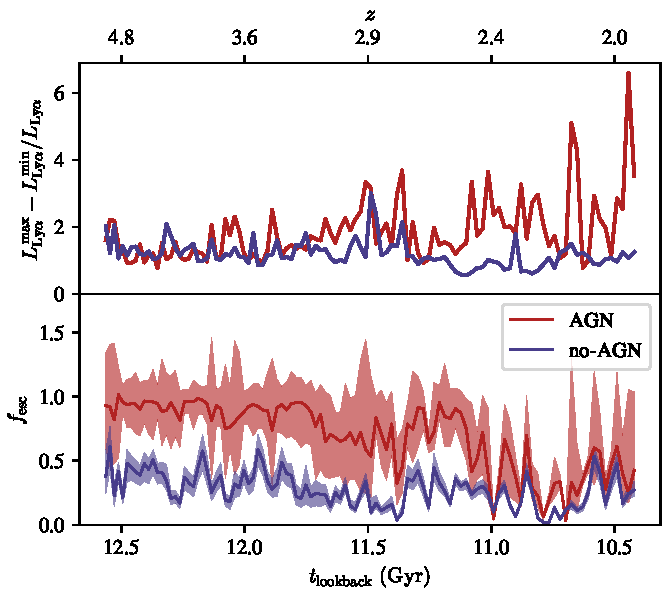
\includegraphics[width=\textwidth,height=\textheight,keepaspectratio]{figures/agn_stats_by_los.pdf}
    \caption{Maximum fractional difference between lines of sight (top) and escape fraction (bottom) over redshift for a MassiveFIRE galaxy that forms a LAB, with and without AGN. The solid lines on the bottom plot show the median escape fraction over all lines of sight and the shaded region around them show the 1-$\sigma$ variation in that quantity over various lines of sight.}
    \label{fig:f_esc}
\end{figure}

\begin{figure}
    \centering
    \includegraphics[width=\textwidth,height=\textheight,keepaspectratio]{figures/many_los.pdf}
    \caption{
        A single snapshot, seen from 12 equally spaced lines of sight.
    }
    \label{fig:many_los}
\end{figure}


\section{The impact of AGN on the spatial extent and concentration of Ly\texorpdfstring{$\alpha$}{a} in blobs}

As in the overall Ly$\alpha$ luminosity, the AGN can also impact the spatial extent of Ly$\alpha$ emission in massive halos. This takes two forms: (1) the total area enclosed within a surface brightness contour and (2) the concentration of Ly$\alpha$ light in the system.  We explore these in turn.

Previously, in Figure~\ref{fig:area_plot}, we examined the size of our model LABs as a function of observation sensitivity (solid lines) in a fiducial model that did not have AGN on.  We now turn to the dashed lines in the same figure where we have included AGN.

We see an enhancement of blob size at high surface brightness cutoffs, which indicates that there are regions that have been substantially enhanced in brightness, but at the same time we see a decrease in blob size at much lower cutoffs. We interpret this effect as a complex interaction of the gas ionization state with escape pathways. As gas becomes more ionized it provides a pathway along which Ly$\alpha$ is likely to escape; it is these pathways that produce the small region(s) of very intense surface brightness. However, the presence of a low-opacity pathway out of the blob decreases the probability that a photon will be scattered out into the extended blob structure before it escapes.

The presence of these small pathways out of blob may be useful to detect the presence of AGN in a blob.
We quantify the concentration of light via a metric analogous to $M_{\rm 20}$ \citep{Lotz2004}, where we compute the fraction of pixels in our surface brightness images containing half the total flux, shown for all our snapshots in Figure~\ref{fig:skewness}.
The primary signature of the AGN's effect is to cause the luminosity to be concentrated in a much smaller area.
While this may seem contradictory to the increase in total luminosity and area enclosed, note that this is a {\it relative} concentration.
That is, while the diffuse emission is still significant, the central emission in the ionized bubble surrounding the AGN dominates when compared to this diffuse halo emission such that the overall concentration decreases dramatically for the AGN-on model.
This metric becomes more effective for identifying AGN with higher-resolution observations (Figure~\ref{fig:MUSE}); the bright patches of our surface brightness images are significantly smaller than the spatial resolution of current telescopes.

%Ideally, we would tie the effect of AGN to both total luminosity and the size of a blob. In \S~\ref{sec:formation_of_labs} we drew some comparisons to observations and Table~\ref{table:labs} we enumerated some known properties of literature LABs. At that stage we were able to avoid defining a strict definition of the size of a blob, but now to clearly discuss the size of a blob we need to pick an surface brightness to consider the edge of a blob; we choose $10^{-18}$ erg/s/cm$^2$/arcsec$^2$. With this as our definition we can see the effect of an AGN on LAB size in Figure \ref{fig:agn_blob_size}. At higher redshifts the AGN provides a notable increase to the size of the blob, but at lower redshifts the AGN effect converges with the no-AGN blob in terms of size.
%\red{not sure why AGN luminosity converges at lower redshift, consider plotting as histogram of area with AGN on and histogram of areas with AGN off}

%We also investigate the effect of an AGN's presence on the distribution of Ly$\alpha$ luminosity across a LAB surface-brighness image. As noted earlier in \S~\ref{sec:formation_of_labs}, metrics for LAB properties that assume azimuthal symmetry are challenging, but also any measurement that requires identification of a center is challenging to apply for the same reason: blobs are amorphous. So as before where we used enclosed area of isphotes which is agonstic to the location and geometry of a blob as opposed to surface brightness profiles, we compute a metric which is notionally similar to $M_{20}$, and plot this to identify snapshots where an AGN's presence becomes visible \ref{fig:skewness}.
%In this plot we have chosen 50\% as the threshold, but this choice is not particular, we could choose any other threshold and see a similar conclusion: The primary signature of an AGN's effect is to cause the luminosity to be concentrated in a much smaller area. Note that in this metric, we do not require that this area be connected; surface brightness images such as that seen in Figure~\ref{fig:agn_on_example} are challenging for other measurements such as a surface brightness profile.

\begin{figure}
  \centering
    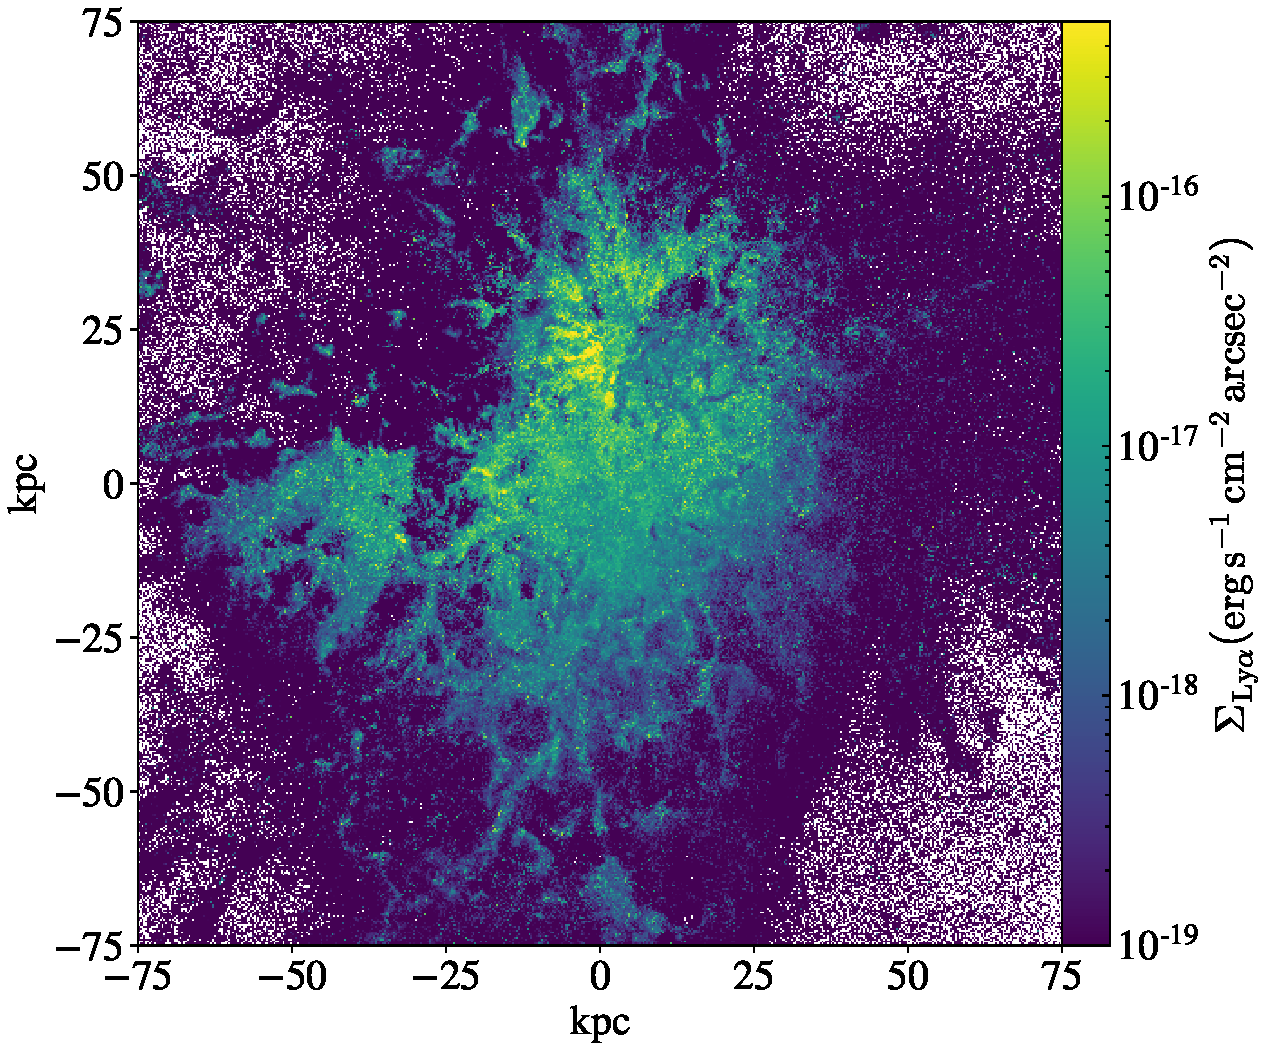
\includegraphics[width=\textwidth,height=\textheight,keepaspectratio]{figures/141.pdf}
  \caption{Example surface brightness image of a LAB where the luminosity is concentrated, which indicates the presence of an AGN, but the luminosity is not in a connected region.}
  \label{fig:agn_on_example}
\end{figure}

\begin{figure}
  \centering
    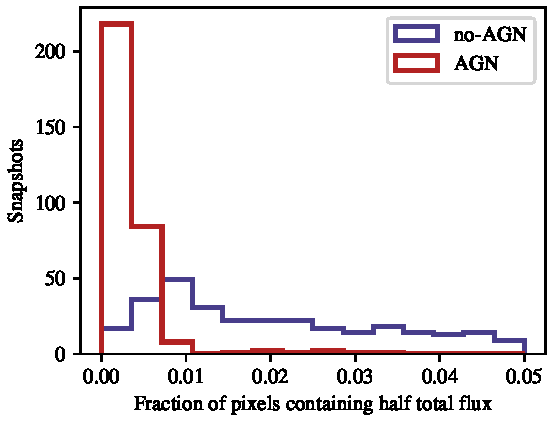
\includegraphics[width=\textwidth,height=\textheight,keepaspectratio]{figures/skew_distribution.pdf}
  \caption{We propose a metric for determining the presence of an AGN in an observed LAB: The fraction of all flux that is concentrated within a small fraction of the total area of the blob. In this figure since we are making a suggestion for an observable metric we have computed this metric on simulated surface brightness images after convolving to the resolution of MUSE. For the purpose of this demonstration we plot the fraction of pixels containing 50\% total flux but one could choose another threshold and find similar results.}
  \label{fig:skewness}
\end{figure}

\section{Impact of AGN model}
